\documentclass[10pt,dvipsnames,svgnames]{beamer}
\setbeamertemplate{navigation symbols}{}
\usepackage{tikzducks,tikzlings}
\usetikzlibrary{decorations.markings,calc}
\usetikzlibrary{shapes,shapes.callouts}
\usetikzlibrary{overlay-beamer-styles} % ich koennte Claudio erwuergen fuer den Namen ;-)
\def\DelayFactor{15}
\tikzset{CastShadow/.style={anchor=south,inner sep=0}}
\newcommand{\CastShadowOutsideTikZ}[2][]{
\begin{tikzpicture}[baseline=(temp.base)]
  \node[CastShadow,#1](temp){#2};
  \node[scope fading=south,opacity=0.4,yscale=-1,CastShadow,#1]{#2};
\end{tikzpicture}
}
\begin{document}
\begin{frame}[plain]
\centering
\CastShadowOutsideTikZ[font=\Huge,text=blue]{Recently in the marmot burrow}
\foreach \X in {1,...,\DelayFactor}
{\only<\X>{}}
\end{frame}

\newcommand\Dialogue[1]{\ifcase#1
\or
Hmmh, I am wondering what ``Eulen nach Athen tragen'' is in
English.
\or
We could ask David.
\or
Better not, he would only ask Google translate.
\or
Nahh, that doesn't look right. 
\or
What?! Carrying coal to Newcastle?
\or
No way we are going there!
\or
Let's go to Athens, Jake, it's time.
\or
OK! Can't wait to get there!
\fi
}


\begin{frame}[t]
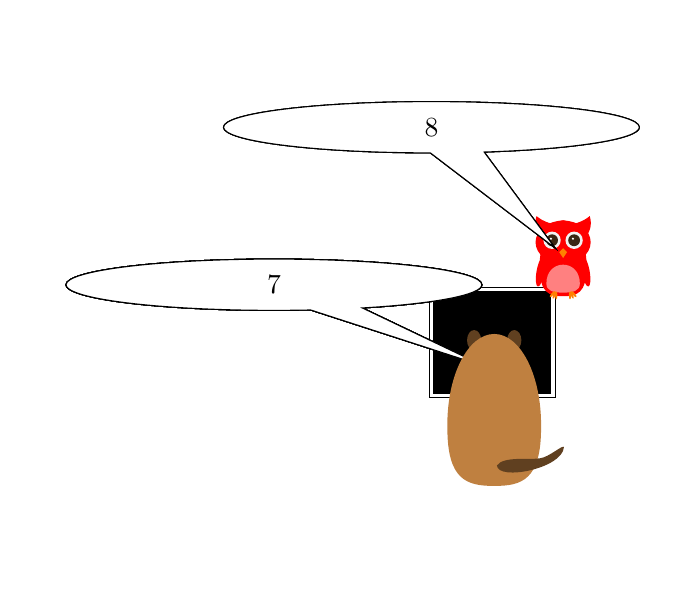
\begin{tikzpicture}
\path[use as bounding box] (-5,6) rectangle (3,-1);
\draw (0.1,1.3) rectangle (1.7,2.7);
\fill (0.15,1.35) rectangle (1.65,2.65);
% Ears %%%%%%%%%%%%%%%%%%%%%%%%%%%%%%%%%%%%%%%%%%%%%%%%%%%%%%%%%%%%%%%
\fill[brown!50!black] (1.18,2.03) ellipse (0.09 and 0.13);
\fill[brown!50!black] (0.67,2.03) ellipse (0.09 and 0.13);
%
\foreach \X [evaluate=\X as \Y using {int((\X-1)*\DelayFactor+1)},
evaluate=\X as \Z using {int(\X*\DelayFactor)}] in {1,3,4,...,7}
{
\node [visible on=<{\Y-\Z}>,ellipse callout, draw,cloud puffs=10,cloud puff arc=120, aspect=2,anchor=south
east,text width=3.5cm,align=center,fill=white,callout absolute pointer={(0.8,1.7)}]
at (0,2.5) {\Dialogue{\X}};
}
% Body %%%%%%%%%%%%%%%%%%%%%%%%%%%%%%%%%%%%%%%%%%%%%%%%%%%%%%%%%%%%%%%
\fill[brown] (1.52,0.92) .. controls (1.52,0.26) and (1.28,0.18) .. (0.925,0.18) .. controls (0.57,0.18) and (0.33,0.26) .. (0.33,0.92) .. controls (0.32,1.58) and (0.59,2.11) .. (0.925,2.11) .. controls (1.26,2.11) and (1.53,1.58) .. (1.52,0.92) -- cycle;
%
% Tail %%%%%%%%%%%%%%%%%%%%%%%%%%%%%%%%%%%%%%%%%%%%%%%%%%%%%%%%%%%%%%%
\fill[brown!50!black] (1.81,0.67) .. controls (1.79,0.40) and (0.97,0.24) ..
(0.96,0.44) .. controls (1.04,0.56) and (1.37,0.51) .. (1.50,0.53) .. controls
(1.62,0.54) and (1.81,0.72) .. (1.81,0.67) -- cycle;
\owl[shift={(1.8,2.5)},scale=0.5,body=red]
\foreach \X [evaluate=\X as \Y using {int((\X-1)*\DelayFactor+1)},
evaluate=\X as \Z using {int(\X*\DelayFactor)}] in {2,6,8}
{\node [visible on=<{\Y-\Z}>,ellipse callout, draw,cloud puffs=10,cloud puff arc=120, aspect=2,anchor=south
east,text width=3.5cm,align=center,fill=white,callout absolute pointer={(1.7,3.2)}]
at (2,4.5) {\Dialogue{\X}};}
\end{tikzpicture}
\end{frame}

\begin{frame}[plain]
\centering
\CastShadowOutsideTikZ[font=\Huge,text=blue]{A bit later in Athens}
\foreach \X in {1,...,\DelayFactor}
{\only<\X>{}}
\end{frame}


\foreach \X [count=\Y] in {0.05,0.06,...,1}
{\begin{frame}[plain]
\hspace*{-1cm}
\begin{tikzpicture}
\node (pic)  {\includegraphics[width=12.2cm]{Athens.jpg}}; % https://cdn.britannica.com/s:700x450/66/102266-004-65D274D5.jpg
%\draw[red,thick] (6,0.4) to[out=-135,in=0] (-1.4,-0.8);
\clip (pic.south west) rectangle (pic.north east);
\draw[decorate,decoration={markings,
mark=at position {\X} with {\coordinate (M) at (0,-0.5);
\pgftransformreset
\path let \p1=(M),\n1={max(0.1,(-0.3*\y1+0.1)/14)} in \pgfextra{\typeout{\X:\n1}
\xdef\myscale{\n1}};
\owl[shift={([yshift=\myscale*1cm]M)},scale=0.5*\myscale,body=red]
\marmot[shift={([yshift=-\myscale*1cm]M)},teeth,whiskers,scale=\myscale]}}]
(6,0.2) to[out=-135,in=0] (-1.4,-1);
\end{tikzpicture}
\end{frame}}
\end{document}


\documentclass[tikz,border=3.14mm]{standalone}
\usepackage{tikzlings}
\end{document}

\begin{tikzpicture}
\draw (-1,-3) rectangle (10,5);
\duck[easter=brown!70!gray,
  egga=blue,
  eggb=green,
  eggc=red]
\coati[sideward,xshift=5cm]
\begin{scope}[xshift=5cm]
\only<1-2>{
\fill (0.5,0.8) -- (-0.1,1) -- (-1,1) -- (-1,1.1) -- (0.5,1.1);}
\only<3-4>{\begin{scope}[rotate around={80:(0,0.8)}]
\fill (0.5,0.8) -- (-0.1,1) -- (-1,1) -- (-1,1.1) -- (0.5,1.1);
\end{scope}}
\end{scope}
\only<1>{
\node[ellipse callout,draw,anchor=south east,align=center,
callout absolute pointer={(4.5,1.5)}] at (4,2) {Give me\\ all
your\\ eggs!};}
\only<2->{
\marmot[xshift=8.5cm,whiskers,teeth]
}
\only<2>{
\node[ellipse callout,draw,anchor=south east,align=center,
callout absolute pointer={(8.2,1.7)}] at (7.5,3) {No no no!};}
\only<3>{
\node[ellipse callout,draw,anchor=south east,align=center,
callout absolute pointer={(8.2,1.7)}] at (7.5,3) {How often do I have to tell
you?!};}
\only<4>{
\node[ellipse callout,draw,anchor=south east,align=center,
callout absolute pointer={(8.2,1.7)}] at (7.5,3) {It is \emph{rubber duck}!\\ 
And not \emph{rob--a--duck}!};}
\end{tikzpicture}
